%Wf4ever Main Document File
\documentclass[a4paper, twoside, 11pt]{article}

\usepackage[scaled=0.92]{helvet}
\usepackage{fancyhdr}
\usepackage{courier}
\usepackage{subfigure}
\normalfont % in case the EC fonts aren't available
\usepackage[T1]{fontenc}
\parskip=2pt\parindent 0pt


\usepackage{url}
\usepackage{hyperref}
\usepackage{wf4ever}
\usepackage{xspace}
\usepackage{amsfonts}
\usepackage{amssymb}
\usepackage{amsmath}
\usepackage{verbatim}

\usepackage{color}
%figure with pdf latex
\usepackage[pdftex]{graphicx}
\usepackage{epstopdf}
\DeclareGraphicsExtensions{.jpg,.pdf,.png}

% Macros

% Identifying documents

\id{2.2v1}
\idyear{2012} %To adjust year for "Document Identifier"
\title{D\delid\ Design, implementation and deployment of workflow
  lifecycle management components - Phase I}
\coordinator{Sean Bechhofer} %Del Coordinator
\institution{University of Manchester} %Del Coordinating Inst.
\authors{Khalid Belhajjame} %Other authors
\abstract{This deliverable describes the first phase of delivery of
  workflow lifecycle management components. It includes a description
  of the Research Object Model, which facilitates interoperation
  between components; an initial Research Object Storage and Retrieval
Service; RO Manager command line tool; and a definition of a model for
workflow abstraction.}
\version{v1.x} %Please fill out version
\datesubmitted{July 31, 2010} %Submission date
\datedue{July 31, 2010} %Date due
\state{Final} %State
\distribution{Public} %Distribution (Public, Restricted, Confidential)

%For Copyrightfooter: Years that copyright should cover, e.g. 2006, 2007, 2006--2007 aso
\copyrighty{2012}



\begin{document}
\maketitle

\section*{Work package participants} The following partners have taken an active part in the work leading to the elaboration of this document, even if they might not have directly contributed to the writing of this document or its parts: %Enter Work Package Participants:
\begin{itemize}
\item iSOCO
\item OXF
\item PSNC
\item UNIMAN
\item UPM
\end{itemize}

\section*{Change Log}
%Fill in table
\begin{centering}

\begin{tabular}{|c|c|p{4.92cm}|p{6.5cm}|}

\hline \textbf{Version} & \textbf{Date} & \textbf{Amended by} & \textbf{Changes} \\ \hline
0.1 & 02-07-2012 & Sean Bechhofer & Initial Version \\ \hline
&&&\\ \hline
&&&\\ \hline

\end{tabular}

\end{centering}
\clearpage
\section*{Executive Summary}
%Please enter Executive Summary
This deliverable describes the first phase of delivery of workflow
lifecycle management components. These components include
\begin{itemize}
\item A description of the Research Object Model. This provides
  vocabularies supporting aggregation and annotation of aggregations
  with specific vocabulary describing workflows and workflow provenance;
\item Services for creating and management of Research Objects (the
  Research Object Storage and Retrieval Service);
\item A command line tool for management of ROs stored locally;
\item A model for workflow abstraction;
\item An initial characterisation of workflow decay.
\end{itemize}
\clearpage

\tableofcontents
\clearpage
\listoftables %Add comment to suppress list of tables
\listoffigures %Add comment to suppress list of figures

\clearpage
\sloppy

%Your work starts here

\section{Introduction}

This deliverable describes aspects of Phase I of the design,
implementation and deployment of the Wf4Ever components that will
support workflow lifecycle management. The document should be read in
tandem with other Month 20 deliverables, in particular
D3.2v1~\cite{D3.2v1} and D4.2v1~\cite{D4.2v1} which adress
complementary aspects of the overall wf4ver architecture and
components.

According to the Description of Work, \emph{This prototype will
  include the following functionalities: an initial Research Object
  model, implemented by means of an ontology network, and basic
  management functions (storage and access), validation
  functionalities based on RO provenance, and definition of semantic
  overlays and workflow provenance matching techniques for
  abstraction.}. 

These requirements are addressed in the following way:

Sections~\ref{sec:model}, \ref{sec:primer} and \ref{sec:examples}
discuss the Research Object Model defined within Wf4Ever along with a
Primer document providing an introduction to that model and a
collection of example Research Objects. 

Sections~\ref{sec:rosrs} and \ref{sec:manager} describe the initial
Research Object Storage and Retrieval Service and Command Line
Manager. Both of these tools use the Research Object Model to
structure the objects that they produce and consume. The RO Model is
thus the ``glue'' that joins together the components and enables
interoperation. 

Section~\ref{sec:abstraction} discusses an initial model for workflow
abstraction, while Section~\ref{sec:decay} presents a characterisation
of workflow decay. 

Note that this document represents the results from Phase I of the
project -- as a result, some areas are not yet complete and we expect
updates, changes and extensions to be reported in Phase II of the
project, due for completion in M32. For example, we expect that RO models reported
here will be subject to change following further usage and experience,
both within and outside the project.

\section{The Research Object Model}
\label{sec:romodel}

The design of the Research object model was informed by a systematic analysis of requirements expressed by scientists from the life sciences and astronomy fields. The results of such analysis are summarised in Figure \ref{fig:wm_abstract}, which distinguishes between core and extended requirements. There are three core requirements that have been identified, namely a mechanism for uniquely identifying Research Objects, a means for aggregating resources within a Research Object, and the ability to annotate the Research Object, its constituent resources and their relationships. Based on the core requirements, the extended requirements highlight the need for specifying workflows (experiments), provenance traces of their executions, the evolution of a Research object over time, as well as mechanisms for citing Research Objects, expressing their dependencies, etc.


\begin{figure}[ht]
  \centering
  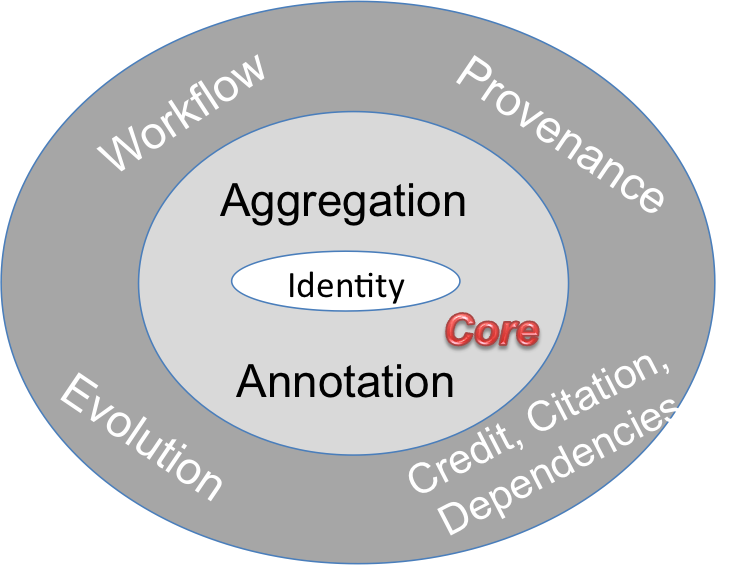
\includegraphics[width=0.4\textwidth]{Figures/wm_abstract.png}
  \caption{Research Objects: Abstract model.}
  \label{fig:wm_abstract}
\end{figure}

We have realized the Research Object abstract model illustrated in Figure \ref{fig:wm_abstract} in the form of a family of ontologies that are illustrated in Figure \ref{fig:wm_concrete}, which we will present in the rest of this section.  It is worth noting that some of the vocabularies, e.g., ORE\footnote{\url{www.openarchives.org/ore}} and OA ~\cite{COG11}, are existing vocabularies that we built on to specify our ontologies.

 \begin{figure}[ht]
  \centering
  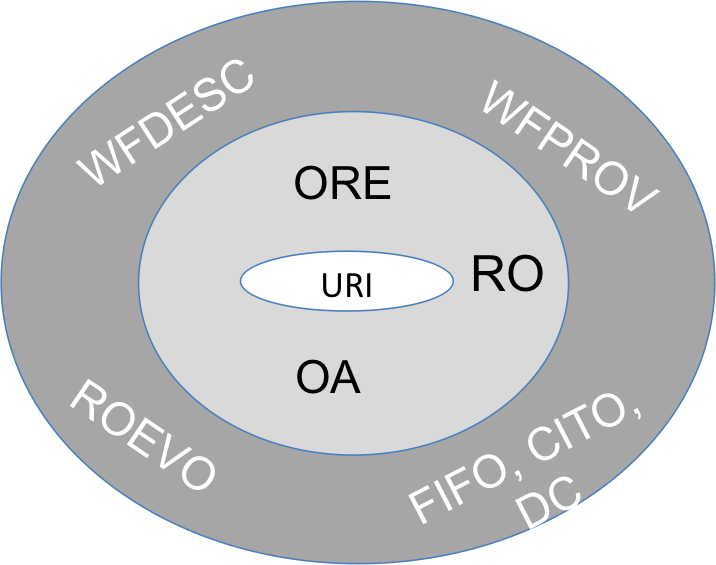
\includegraphics[width=0.4\textwidth]{Figures/wm_concrete.png}
  \caption{Research Objects: Concrete model.}
  \label{fig:wm_concrete}
\end{figure}

\subsection{RO core ontology} 
The Core RO Ontology provides the minimum terms that are essential to the specification of research objects. Specifically, it caters for two essential requirements by providing a container structure that can be used by the scientists to bundle the resources and material relevant for their investigation, and by enabling annotations of such a container, its resources, as well as the relationships between resources thereby making the research object interpretable and reusable. 

To cater for the specification of aggregation structures, we built the Research Object Core Ontology upon the popular ORE vocabulary. ORE defines standards for the description and exchange of aggregations of Web resources. 
Figure \ref{fig:ro_ontology} illustrates the main terms that constitute the Research Object Core Ontology, which we describe in what follows.


\begin{figure}[ht]
  \centering
  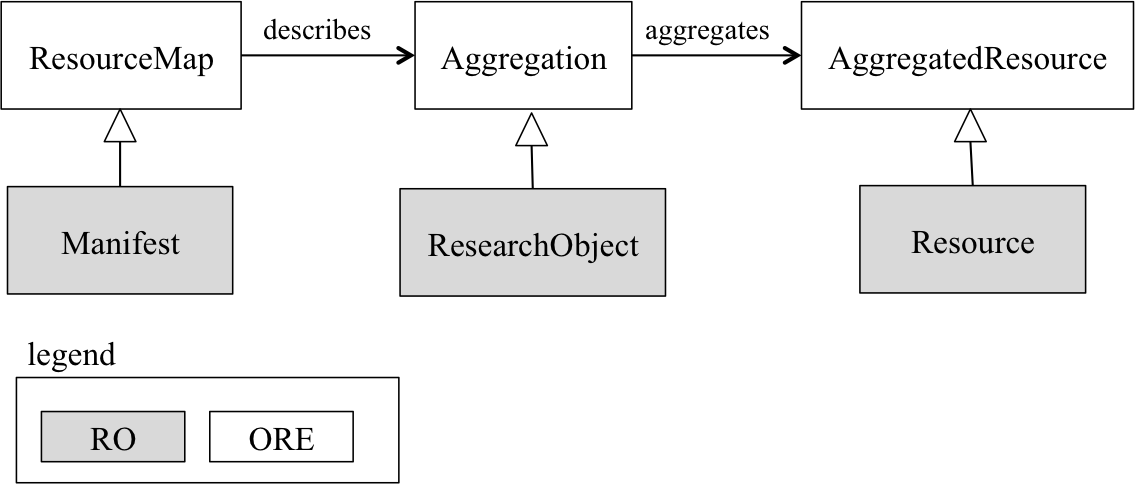
\includegraphics[width=0.6\textwidth]{Figures/ro_ontology_1.png}
  \caption{RO as an ORE aggregation.}
  \label{fig:ro_ontology}
\end{figure}

\begin{itemize}
\item
\texttt{ro:ResearchObject}\footnote{The namespace of the Research Object Core Ontology \texttt{ro} is \url{http://purl.org/net/wf4ever/ro\#}}, represents an aggregation of resources. It is a sub-class of \texttt{ore:Aggregation} and acts as an entry point to the research object.
\item
\texttt{ro:Resource}, represents a resource that can be aggregated within a research object and is a sub-class of \texttt{ore:AggregatedResource}. A resource can be a Dataset, Paper, Software or Annotation. Typically, a \texttt{ro:ResearchObject} aggregates multiple \texttt{ro:Resource}, and this relationship is specified using the property \texttt{ore:aggregates}.
\item
\texttt{ro:Manifest}, a sub-class of \texttt{ore:ResourceMap}, represents a resource that is used to describe a \texttt{ro:ResearchObject}. It plays a similar role to the manifest in a JAR or a ZIP file, and is primarily used to list the resources that are aggregated within the research object.
\end{itemize}

The second core requirement that, the Research Object Core Ontology caters for, is the descriptions of the research object and its elements. We chose the Annotation Ontology (AO) release 2.0b2~\cite{COG11}.To annotate research objects, we make use of the following three Annotation Ontology terms \texttt{ao:Annotation}\footnote{The namespace of \texttt{ao} is \url{http://purl.org/ao/}}, which represents the annotation itself; \texttt{ao:Target}, which is used to specify the \texttt{ro:Resource}(s) or \texttt{ro:ResearchObject}(s) subject to annotation; and \texttt{ao:Body}, which comprises a description of the target.
In the case of research objects, we use annotations as a mean for decorating a resource (or a set of resources) with metadata information. The body is specified in the form of a set of RDF statements, which can be used to, e.g., specify  the date of creation of the target or its relationship with other resources or research objects. Also, annotations can be provided for human consumption (e.g. a description of a hypothesis that is tested by a workflow-based experiment), or for machine consumption (e.g. a structured description of the provenance of results generated by a workflow run). Both kinds of annotations are accommodated using Annotation Ontology structures.

\subsection{RO Extension Ontologies}
We present in this section two  extensions to the core Research Object ontology. The first specializes the kinds of resources that the research object can aggregate. In particular, we present extensions to specify  method and experiments and the traces of their executions. The second kind of extension shows how specific metadata information, specifying the evolution of the research object over time, can be specified by specializing the Research Object core ontology.

\paragraph{Specifying Workflows}
To describe workflow research objects the workflow description vocabulary \textit{wfdesc}\footnote{The name space of \textit{wfdesc} is \url{http://purl.org/wf4ever/wfdesc\#}.} defines several specific resources that are involved in a workflow specification. The choice of these resources was performed by examining the commonalities between major data driven workflows, namely Taverna\footnote{http://www.taverna.org.uk}, Wings\footnote{http://http://wings-workflows.org} and Galaxy\footnote{http://galaxyproject.org}, to cite a few.

\begin{figure}[ht]
  \centering
  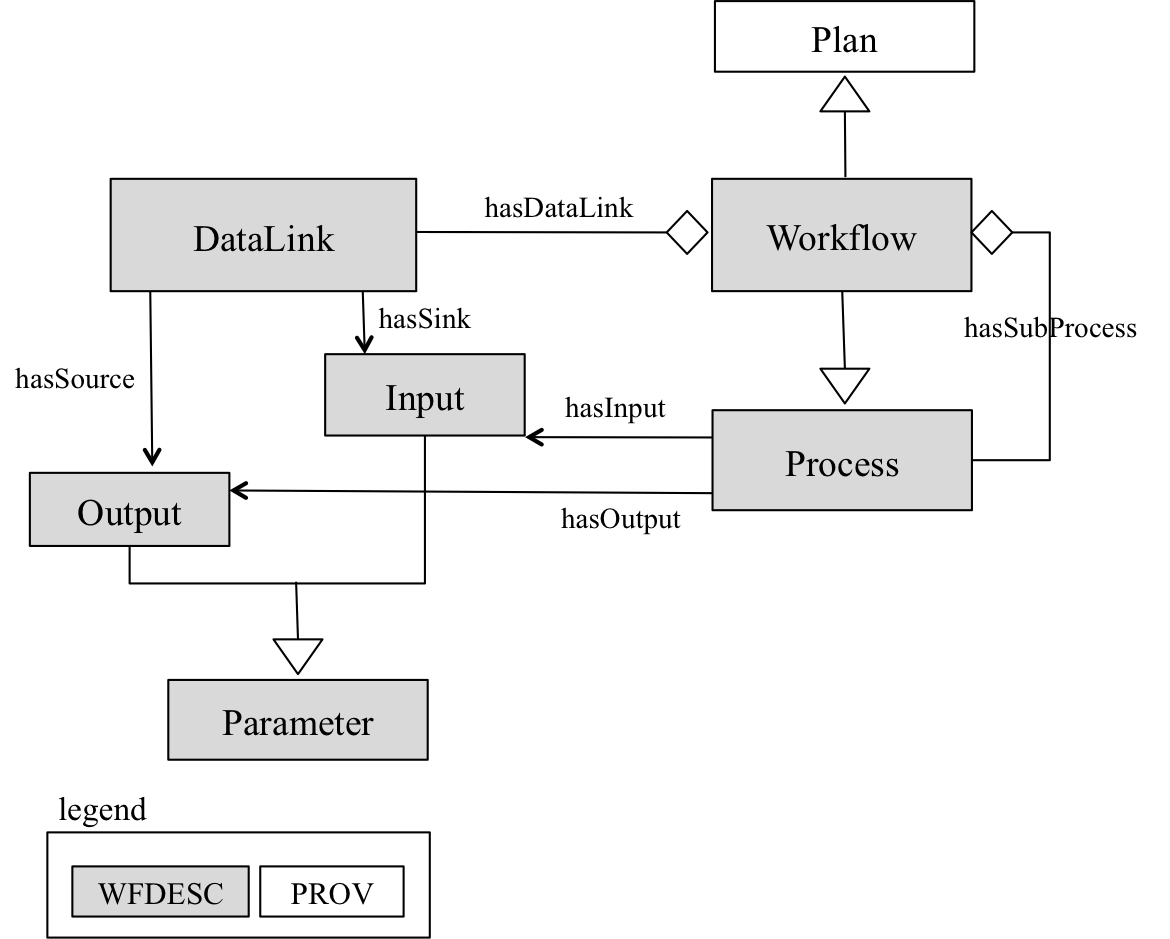
\includegraphics[width=0.6\textwidth]{Figures/wfdesc.png}
  \caption{The \textit{wfdesc} ontology.}
  \label{fig:wfdesc}
\end{figure}

Figure \ref{fig:wfdesc} illustrates the terms that compose the \textit{wfdesc} ontology. Using such ontology, a workflow is described using the following three main terms:
\begin{itemize}
\item
\texttt{wfdesc:Workflow} refers to a network in which the nodes are processes and the edges represent data links. It is defined as a subclass of the \textit{Plan} concept from the PROV-O ontology, which represents a set of actions or steps intended by one or more agents to achieve some goals \cite{w3c-prov-o}. 
\item
\texttt{wfdesc:Process} is used to describe a class of actions that when enacted give rise to process runs. Processes specify the software component (e.g., web service) responsible for undertaking those actions.
\item
\texttt{wfdesc:DataLink} is used to encode the data dependencies between the processes that constitute a workflow. Specifically, a data link connects the output of a given process to the input of another process, specifying that the artifacts produced by the former are used to feed the latter.
\end{itemize}


\paragraph{Describing Experimental Provenance using the \textit{wfprov} Vocabulary}
The \textit{wfprov} ontology is used to describe the provenance traces obtained by enacting  workflows. It is defined as an extension to the ongoing W3C PROV standard ontology - PROV-O\footnote{Note that the \textit{wfprov} is reported in the W3C PROV Working Group implementation report.}.

\begin{figure}[ht]
  \centering
  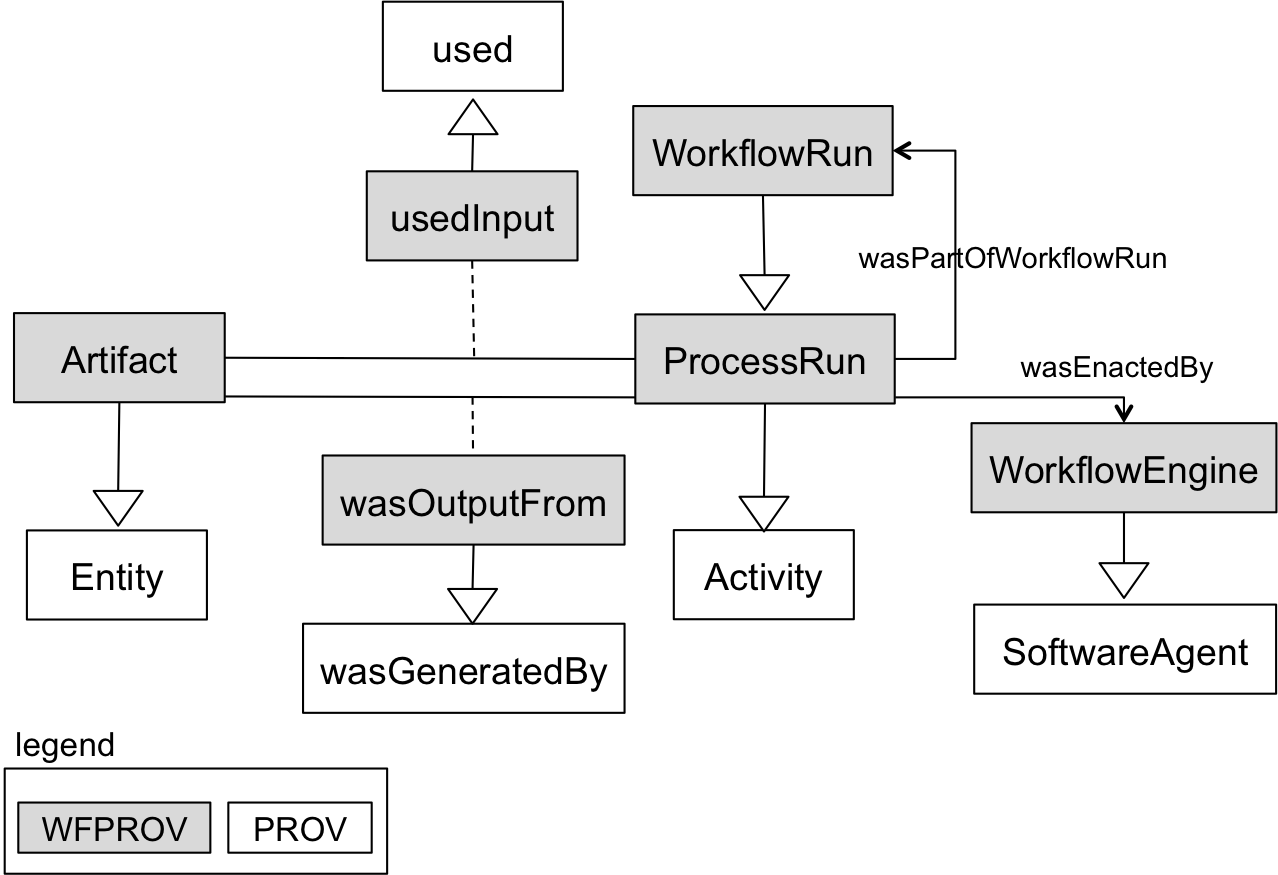
\includegraphics[width=0.6\textwidth]{Figures/wfprov.png}
  \caption{The \textit{wfprov} ontology.}
  \label{fig:wfprov}
\end{figure}

Figure \ref{fig:wfprov} illustrates the structure of the \textit{wfprov} ontology and its alignments with the W3C PROV-O ontology. A a workflow run~(\texttt{wfprov:WorkflowRun}) represents the enactment of a given workflow. It is composed of a set of process runs~(\texttt{wfprov:ProcessRun}), each representing the enactment of a process. A process run may use some artifacts~(\texttt{wfprov:Artifact}) as input and generate others as output. A process run is enacted by a workflow engine~(\texttt{wfprov:WorkflowEngine}), which can be seen as a PROV software agent.

By chaining the usage and generation of artifact together, the \textit{wfprov} ontology allows scientists to trace the lineage of workflow results. For example the user can identify the input artifacts that were used to feed the wokflow run (as a whole) to obtain a given output that was generated by the workflow run.

\paragraph{Tracking Research Object Evolution using the \textit{roevo} Vocabulary}
The \textit{roevo} ontology is another extension to the minimal core ontology for describing an important aspect of research objects, its life cycle.
%There are a number of existing work captures changes of information objects, like the changeset vocabulary, evolution of ontologies, like xxx, yyy, etc. 
To track the life cycle of a research object, we need to describe its changes at different levels of granularity, about the research object as a whole and about the individual resources. Also, we want to provide sufficient details to track the changes in order to roll back to a particular version or to quality control changes. Therefore, we need to describe when the change took place, who performed the change, and dependency relationships between the changes. %None of the existing vocabularies provide all the structure for us to build upon. 
Change is closely related to the provenance of a particular version of a research object or a resource. A study of the latest PROV-O ontology shows that it indeed provides all the foundational information elements for us to build the evolution ontology. 

\begin{figure}[ht]
  \centering
  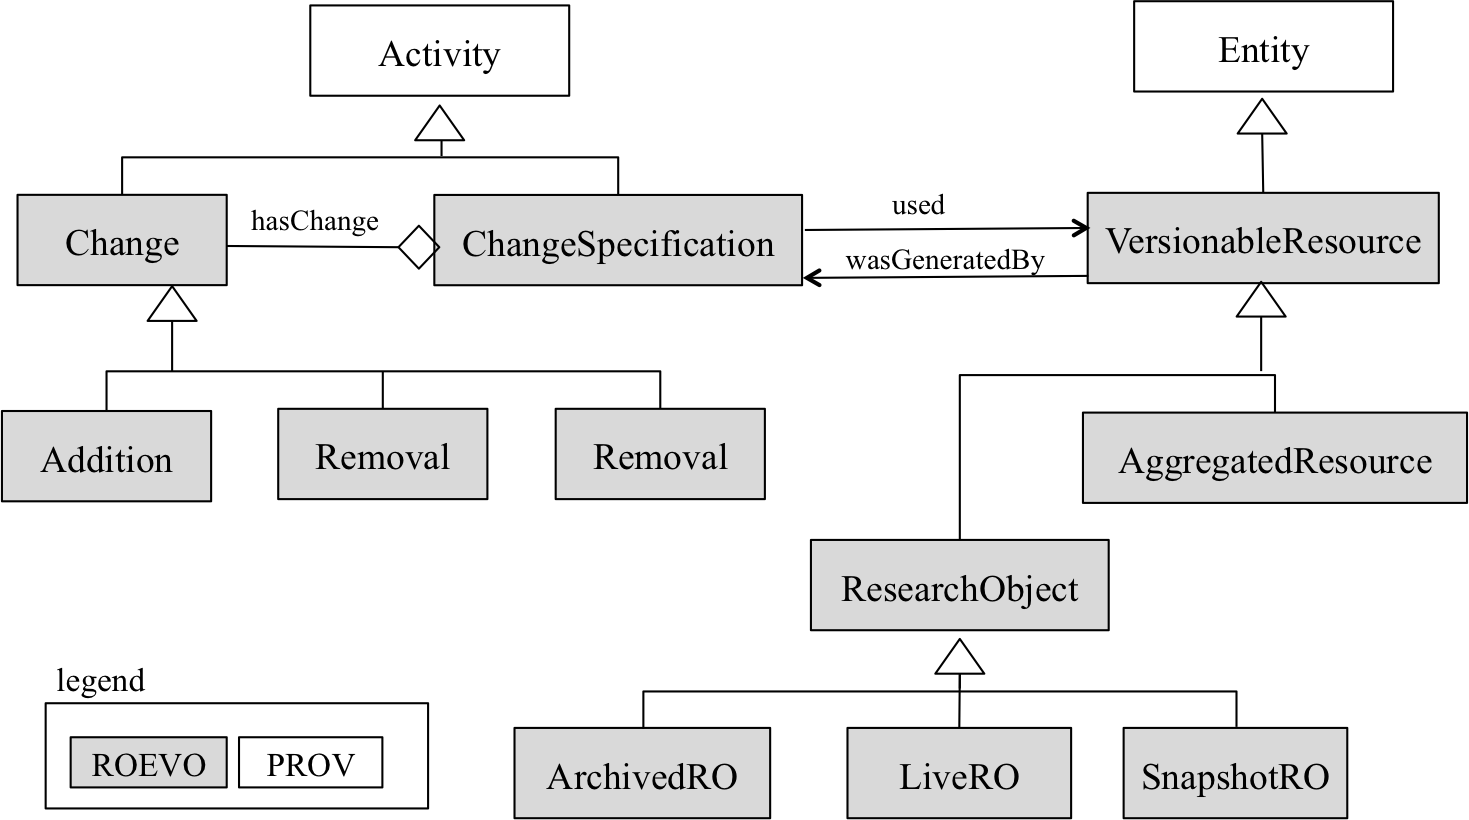
\includegraphics[width=0.6\textwidth]{Figures/roevo.png}
  \caption{The \textit{roevo} ontology extending PROV-O core terms.}
  \label{fig:ro_evo}
\end{figure}    

Figure~\ref{fig:ro_evo} illustrates the core concepts of this ontology and how it extends the PROV-O:
\begin{itemize}
\item To capture different status of a research object we create three sub-classes of \texttt{ro:ResearchObject}: the \texttt{roevo:LiveRO} is a research object to capture research findings during a live investigation and it can changed, and it can either archived or snapshotted. The \texttt{roevo:ArchivedRO} can be regarded as a production research object to be preserved and archived, such as one describing findings published in an article, and it can no longer be changed; the \texttt{roevo:SnapshotRO} represents a live Research Object at a particular time.
\item Both a snapshot of a live Research Object and an archived Research Object can be regarded as a versioned Research Object, i.e. a \texttt{roevo:VersionableResource}, Because it is a sub-class of \texttt{prov:Entity}, we can reuse PROV-O properties to describe the provenance or changes of this entity, such as pointing to the activity leading to any of its changes, the source research object that it was derived from, and the agent involved in its change.
\item A change is a \texttt{prov:Activity}, which means that it has a start time, an end time, an input entity and a resulting entity. Also a change leading to a new Research Object can constitute a series of changes. Therefore, we have a composite \texttt{roevo:ChangeSpecification} activity, which has a number of unit \texttt{roevo:Change}s. A unit change can be adding, removing or modifying a resource or a research object. But these different changes share the same pattern of taking an input entity and producing an output entity, which can all be nicely covered by properties from PROV-O.
\end{itemize}

As well as the above vocabularies, the Research Object model makes use of existing vocabularies, in particular, FOF\footnote{\url{http://xmlns.com/foaf/spec/}}, DCTerms\footnote{\url{http://dublincore.org/documents/dcmi-terms/}}, CITO\footnote{\url{http://vocab.ox.ac.uk/cito}}, and SCIOC\footnote{\url{http://sioc-project.org/ontology}} to provide Research Objects designers with the means to expresse aspects such as the people who were involved in the creation of a Research Object, its citation, as well as dependencies that the Research Object may have. For instance, we make use of the term \texttt{dc:requires} to specify that a the execution of a workflow requires other resources, e.g., plugins, credential, or specific execution environment.


\section{Research Objects Primer}
\label{sec:primer}

The Research Object Ontologies and Vocabularies Primer is a document
targeted at users, providing an accessible introduction to the Wf4Ever
RO Model. This will enable readers to understand \emph{what} the RO Model
provides and \emph{how} the RO Ontologies and Vocabularies can be used to
describe an aggregation object that represents scientific experiments
in a structured format. 

The document is published online at \url{http://wf4ever.github.com/ro-primer/}



\section{Research Object Examples}
\label{sec:examples}

A number of exemplar Research Objects have been described. These provide illustrative examples of how the model may be used to describe aggregations of content. 

\section{Research Object Storage and Retrieval Service}
\label{sec:rosrs}

The Wf4ever Research Objects Digital Library (RODL) will provide a number of services that support the creation, management and manipulation of Research Objects (ROs). Among these services is Storage and Retrieval -- referred to here as ROSRS. 

The ROSRS is provided as a RESTful interface, providing the following functionality:

\begin{itemize}
\item Storing and retrieving research objects;
\item Storing and retrieving resources aggregated within the research objects;
\item Annotating the aggregated resources, including the research object itself. 
\end{itemize}

The ROSRS uses the RO Model (as discussion in Section~\ref{sec:model} to structure and describe the objects it creates. 

Further information describing the details of the ROSRS API are contained in D1.2v1~\cite{D1.4v1}.




\section{Research Object Manager}
\label{sec:manager}

The Research Object Manager provides a command line tool for creating, displaying and manipulating Research Objects. The RO Manager functionality is complementary to that provided by the ROSRS described in Section~\ref{sec:rosrs}. In particular, the RO Manager is primarily designed to support a user working with ROs in the host computer's local file system, with the intention being that the ROSRS and RO Manager can exchange ROs between them -- in part facilitated by the use of the shared RO vocabulary and model.

Past experience has suggested that lightweight, command line tools give users early access to functionality and provide an opportunity to gather additional feedback and requirements on that functionality. Command line tools can also be used with built in operating system functionalty as pipes and input/output redirection in order to quickly build prototype tool chains.

The RO Manager allows users to 
\begin{itemize}
\item Create local ROs;
\item Add resources to an RO;
\item Add annotations to an RO;
\item Read and write ROs to the RODL.
\end{itemize}

As with the ROSRS, the RO Manager uses the RO Model to structure and describe the objects it creates.

Further information describing the details of the RO Manager are contained in D1.4v1 (Reference Wf4Ever Implementation -- Phase I)~\cite{D1.4v1}.


\section{Workflow Abstraction}

\label{sec:abstraction}
The main purpose of the work done so far for workflow abstraction is related to the creation of a trie structure which captures the sequences of execution of a workflow and keeps track of their statistics. A trie is an ordered tree that stores a dynamic set of keys which they usually are strings. For our purposes we have used it for storing the workflow execution in an ordered way by including at different levels of the tree the different inputs, processes and outputs (resources) which are run. Therefore all the descendants of a node have a common prefix of the resource associated with that node. This is very useful for detecting common parts of different workflows because we can easily keep track of the number of times that an specific sequence of resources has been executed. \\

The goal of making an abstraction of a workflow is to make them more reusable as a whole or some parts of it. Then, we define abstraction as the pattern that appears when a sequence of resources are executed together by a minimum number of times. This definition leads also to the concept of pattern or macro identification which applied to workflows leads to finding common sub-workflows. \\ 

The presented work is a bottom-up approach in order to study the actual provenance of workflow results (which represents the dataflow of an executed workflow described in D4.2v1) from a set of available workflows at WINGS~\footnote{\url{http://wings.isi.edu/}} and Taverna~\footnote{\url{http://www.taverna.org.uk/}} created for this purpose. The description of the provenance of workflow results and \textbf{wfprov} ontology can be found at~\cite{D4.2v1} and \footnote{\url{http://purl.org/wf4ever/wfprov#}} respectively, and an example of a RO containing the provenance of workflow results for the Protein Discovery Workflow is available \footnote{\url{http://sandbox.wf4ever-project.org/portal/ro?0&ro=http://sandbox.wf4ever-project.org/rosrs5/ROs/wf74/}} which is part of the RO testbed \footnote{\url{http://www.wf4ever-project.org/wiki/display/docs/RO+testbed}}. \\


This study uses the provenance of the workflow results of different workflows as inputs for creating the trie structure introduced above. Every time a resource is executed its associated node in the trie structure is updated by increasing the number of times that it has been used and afterwards an analysis of the trie can be done to obtain the most common set of resources or macros. \\
 

Though this is still a preliminary work, once a set of macros have been identified it would be possible to categorize them (manually or automatically e.g. by using workflow tags) and afterwards create the associated taxonomy by using the trie membership relations.

The use of the provenance of the workflow results seems to be more appealing that using the workflow templates, which are the static description of a workflow, mainly due to it representing the workflows which are actually running and being used, and also allows to undo control structures as e.g. "if".

The code developed for the creation and maintenance of the trie structure and for accessing to the provenance of the workflow results repository is available at \footnote{\url{https://github.com/wf4ever/wf-abstraction}} and provides the following functionality:

\begin{itemize}
\item It stores the provenance of the workflow results in an ordered way and the appearance frequency of their resources
\item It calculates relative frequencies at different levels of the trie
\item It provides different modes to traverse the structure (pre-ordered/level-ordered)
\item It provides an output XML structure with relative frequencies per level and per process (an output example is available at \footnote{\url{https://github.com/wf4ever/wf-abstraction/blob/master/outputExample.xml})}
\end{itemize}

The Figure~\ref{fig:workflowAbstraction} shows the overall discovery process introduced in this section. The inputs have been obtained by using workflows from WINGS and Taverna and transforming them into \textbf{wfdesc} and \textbf{wfprov} vocabularies to get the provenance of workflow results. That provenance has been stored in a trie structure which captures the order of the executed resources and stores the frequencies of appearance. Then, that information can be used to obtain the most frequent set of ordered executed resources which we have called macros and are identified in the figure of the bottom by black squares. Afterwards these detected macros, which represent some common workflow structures, could be hand-annotated in order to tag them or could be annotated automatically for example by assigning to them the same tags as the workflows that they belong to. Finally a taxonomy which includes all the identified macros by membership (bigger macros contain the smaller ones) will be created for indexing.

\begin{figure}
\begin{center}
	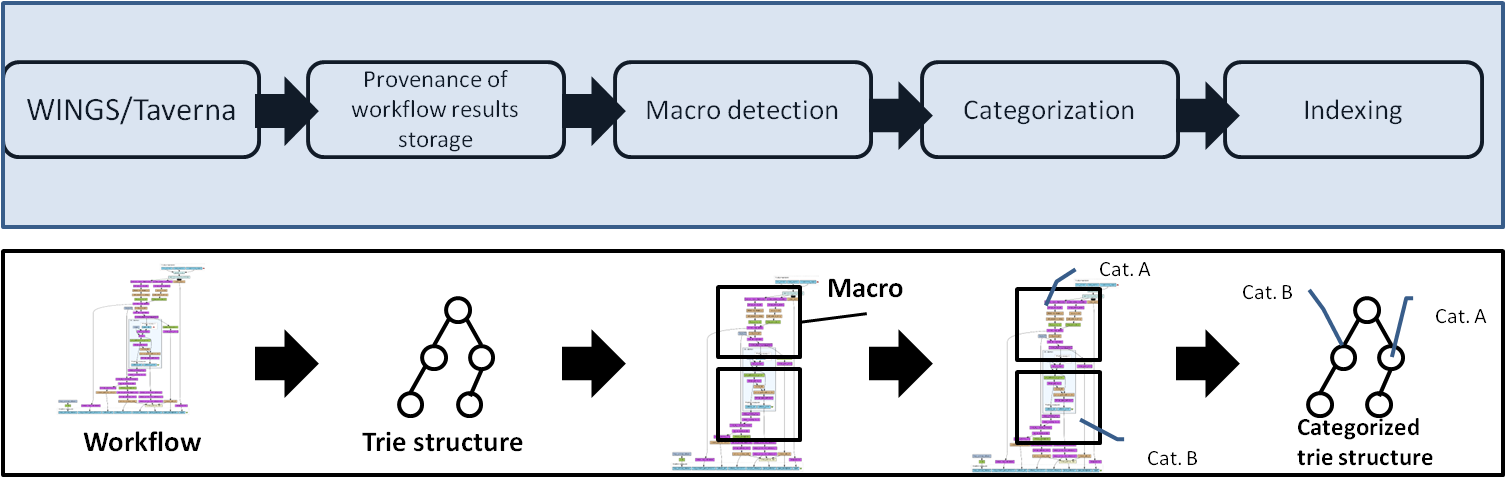
\includegraphics[scale=0.5]{./Figures/workflowAbstraction}
		\caption{Workflow Abstraction Discovery Process}
		\label{fig:workflowAbstraction}
\end{center}
\end{figure}

\section{Characterising Workflow Decay}
\label{sec:decay}

The main impediment to workflow preservation is workflow decay. Indeed, our experience with scientific workflows suggests that a large proportion of workflows suffer from decay \cite{DBLP:conf/eScience/Belhajjame07}, which decreases their value over time. Broadly speaking, we can distinguish two forms of decay. i)- {\bf Inability to re-execute the workflow}: due to many factors, including the unavailability of third party resources that are responsible for executing the tasks that compose the workflows, we may not be able to re-execute a given workflow. ii)- {\bf Inability to reproduce workflow results}: a less severe, yet relevant, form of decay, is the inability to obtain the same (or similar) results when re-executing the workflow. Reproducing previous results can be primordial in reinforcing trust in scientific results and can be used in peer-reviewing as a mechanism to validate the results claimed by given scientists \cite{DBLP:journals/pvldb/FreireBS11,carole2011}. 

The above discussion raises the following question. {\em What are the causes of workflow decay?} To identify and characterise the causes of workflow decay, we adopted a bottom-up approach, whereby we manually analyzed $92$ Taverna workflows from the myExperiment repository. We chose Taverna workflows because they form the largest available workflow collection (more than half of the workflows in myExperiment are Taverna workflows at the time of writing), and Taverna workflows have been published on myExperiment since its launch in 2007, therefore providing a good insight into decay over those years. 

To base our analysis on a sample of workflows that is representative of the set of workflows in myExperiment, we selected workflows using the following three criteria: 
\begin{itemize}
\item
The year of creation of the workflow: we believe that the decay of workflows could be directly impacted by the year of their creation, hence we tried to make an even coverage of Taverna 1 workflows \cite{DBLP:journals/bioinformatics/OinnAFMSGCGPWL04} and Taverna 2 workflows \cite{DBLP:conf/ssdbm/MissierSOTNDWOG10} between the years 2007 and 2012.
\item
The creator of the workflow:  in order to reduce possible bias introduced by specific workflow creators, we avoided choosing workflows created by the same person in the same year.
\item
The domain of the workflow: our workflow selection also had a good coverage of domains, covering $18$ different scientific (such as life sciences, astronomy and cheminformatics) and non-scientific domains (such as testing of Grid services).  Figures \ref{fig:domain_distribution} illustrates the domains of the workflows that we selected for decay analysis.
\end{itemize}
 
 \begin{figure}[h]
  \begin{center}
    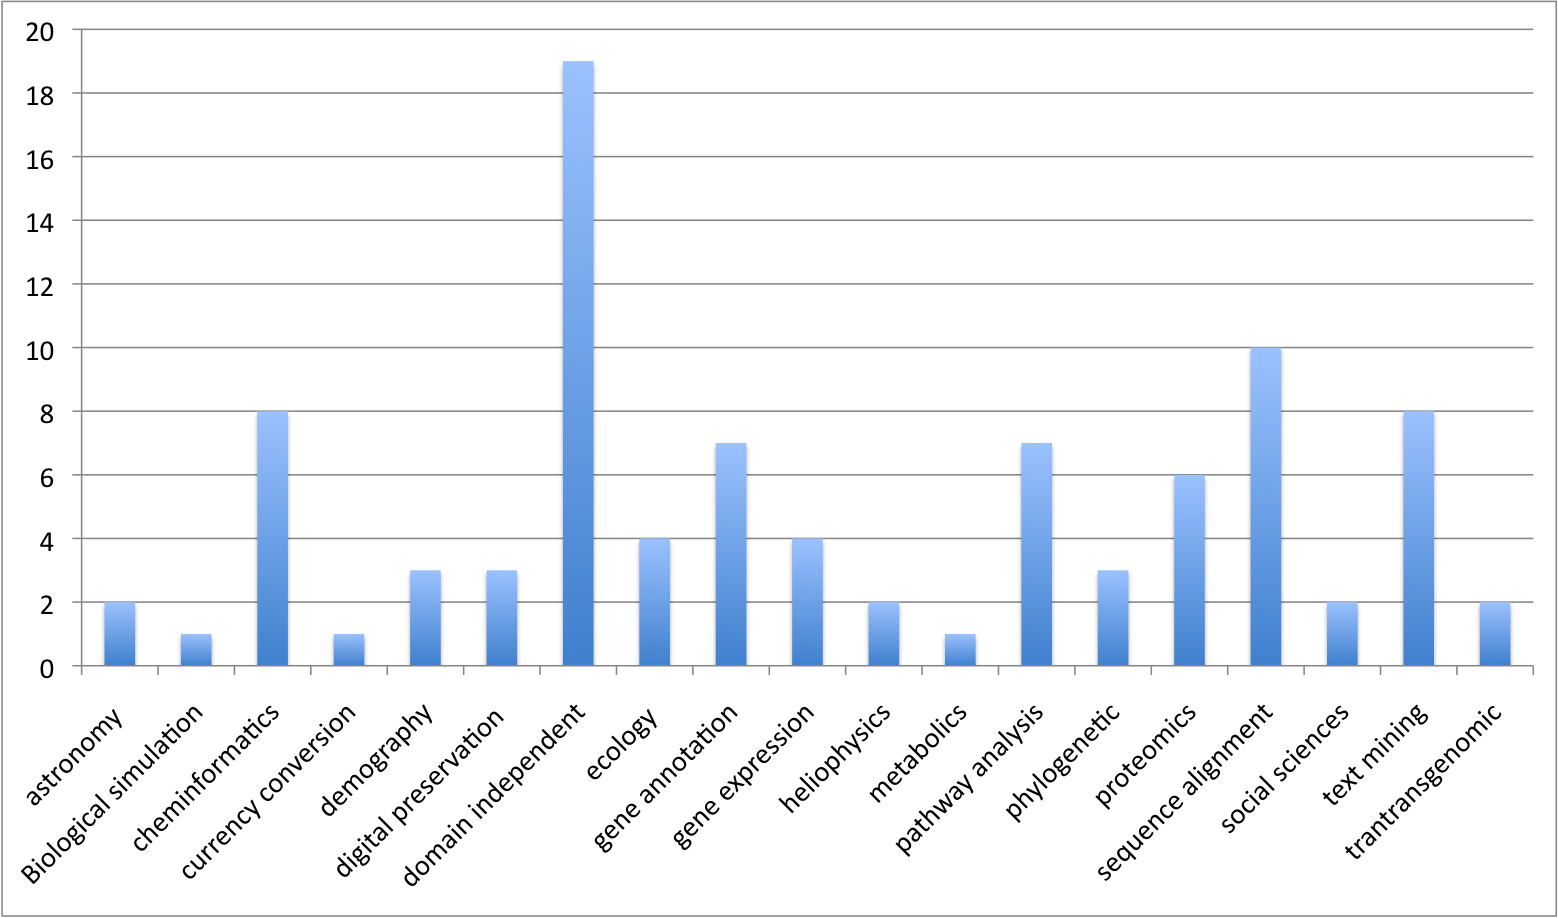
\includegraphics[width=13cm]{./Figures/domain-features.png}
        \caption{Distribution of the domain studied by our test workflows.}
        \label{fig:domain_distribution}
  \end{center}
\end{figure}


Although we focus on a particular family of workflows, i.e., Taverna workflows, we expect our approach and analysis to be applicable to many others and our analysis to be repeatable on a different corpus of workflows. 

To identify the causes of decay that the workflows we selected may suffer from, we attempted to execute them using the Taverna 2.3 workbench. We then manually examined their results, diagnosed broken links, etc. Our analysis showed that nearly $80\%$ of the tested workflows failed to be either executed or produce the same results, and those from earlier years (2007-2009) had more than 80\% failure rate (as shown in Figures~\ref{fig:taverna-wf-failed}). The causes of workflow decay can be classified into four categories, which we present in the rest of this section. 

% \begin{figure}[h]
%   \centering
%   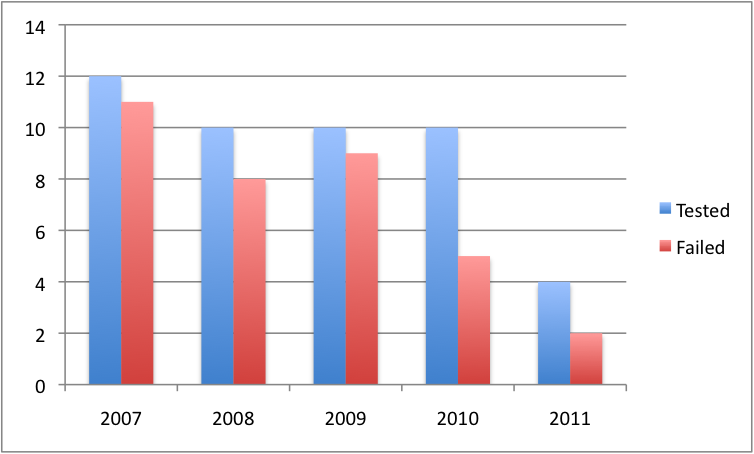
\includegraphics[width=7cm]{./Figures/taverna1-workflows-rate.png}
%   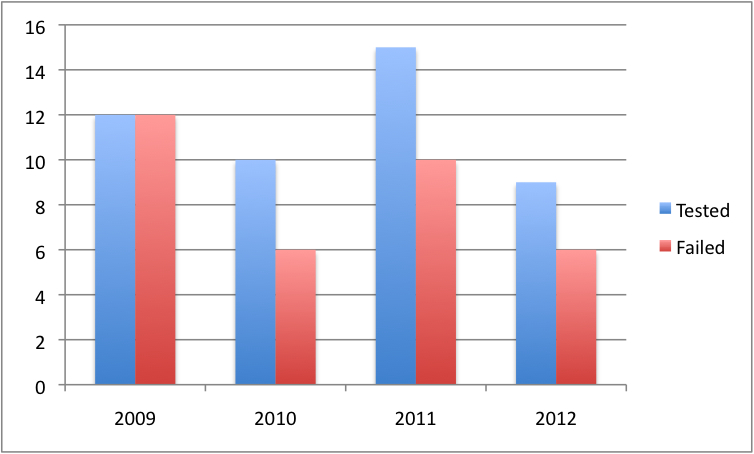
\includegraphics[width=7cm]{./Figures/taverna2-workflows-rate.png}
%  \caption{Number of Taverna workflows tested and failed (Taverna 1 on the left, Taverna 2 on the right)}
%  \label{fig:taverna-wf-failed}
% \end{figure}

\begin{figure}[h]
  \centering
  \begin{subfigure}[t]{9cm}
    \centering
    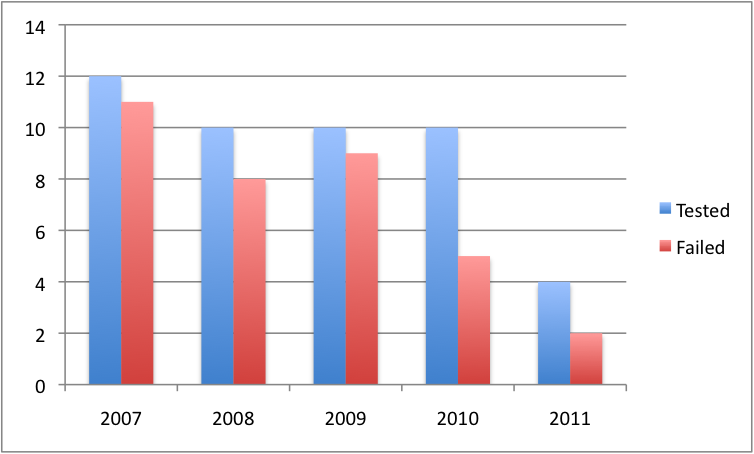
\includegraphics[width=7cm]{./Figures/taverna1-workflows-rate.png}
    \caption{Number of Taverna 1 workflows tested and failed between 2007-2009.}
  \end{subfigure}
  \begin{subfigure}[t]{9cm}
    \centering
    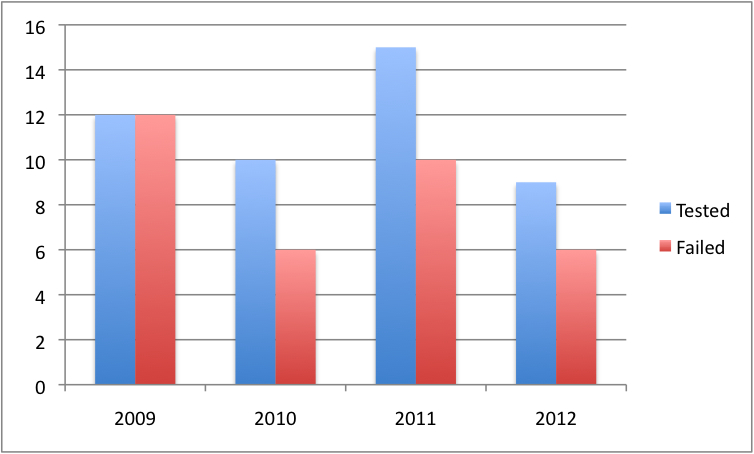
\includegraphics[width=7cm]{./Figures/taverna2-workflows-rate.png}
    \caption{Number of Taverna 2 workflows tested and failed between 2009-2012}
  \end{subfigure}
  \caption{Number of Taverna workflows tested and failed}
  \label{fig:taverna-wf-failed}
\end{figure}

  % \begin{figure}[h]
  % \centering
  % \subfigure[Number of Taverna 1 workflows tested and failed between 2007-2009.]{
  % 	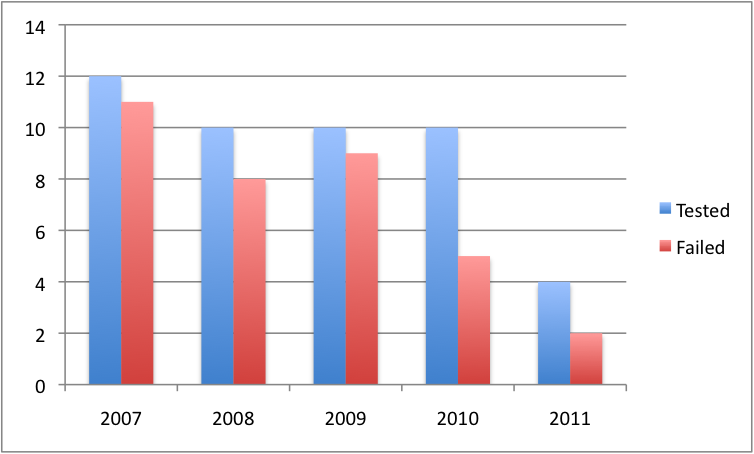
\includegraphics[width=7cm]{./Figures/taverna1-workflows-rate.png}}
  % \subfigure[Number of Taverna 2 workflows tested and failed between 2009-2012.]{
  %     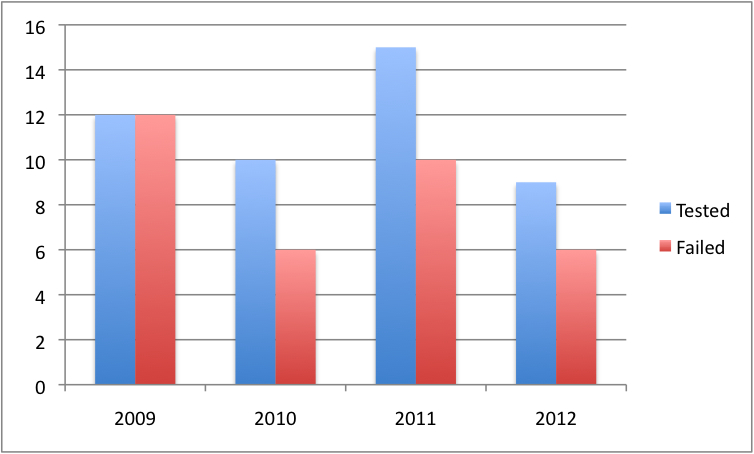
\includegraphics[width=7cm]{./Figures/taverna2-workflows-rate.png}}
  % \caption{Number of Taverna workflows tested and failed}
  % \label{fig:taverna-wf-failed}
  % \end{figure}


\subsection{Volatile third-party resources}
Most of the workflows that we analysed make use of third-party resources such as web services and databases.
The provision of such resources may be interrupted or changed, causing failure of the workflow to execute. In certain cases, the workflow cannot be run, even when the third party resources that it relies on are available, e.g.,  when such resources require authentication. Another cause that may lead to workflow decay, is changes to third party resources. For example, if the web service provider decides to change the implementation of the web service, then the workflow execution may not deliver the same results, or worse, it may not be possible to execute. Table~\ref{table:decay} summarises these causes of decay with concrete examples.


\begin{table}[ht]
\caption{Categorisation of Decay Caused by Third-party Resources} % title of Table
\centering  % used for centering table
\begin{tabular}{p{1.6in} p{2.2in} p{2.2in}} % centered columns (4 columns)
\hline\hline                        %inserts double horizontal lines
Causes &  Refined causes & Examples \\
\hline                  

Third party resources are not available & Underlying datasets, particularly those locally hosted in-house datasets, are no longer available & Researcher hosting the data changed institution, server is no longer available 
\\ \cline{2-3} 
			 									& Services are deprecated & (DNA Data Bank of Japan) DDBJ web services are not longer provided despite the fact that they are used in many myExperiment workflows
 \\ \hline

Third party resources are available but not accessible & Data is available but identified using different IDs than the one known to the user & Due to scalability reasons the input data is superseded by a new version making the workflow not executable or providing wrong results
\\ \cline{2-3}

								& Data is available but permission, certificate, or network to access it is needed & Cannot get the input, which is a security token that can only be obtained by a registered user of ChemiSpider
\\ \cline{2-3}
								& Services are available but need permission, certificate, or network to access and invoke them	& The security policies of the execution framework are updated due to new hosting institution rules \\
\hline
Third party resources have changed &  Services are still available by using the same identifiers but their functionality have changed & The web services are updated intentionally or unintentionally (e.g.malware) providing wrong results \\
\hline
\end{tabular}
\label{table:decay} % is used to refer this table in the text
\end{table}

\subsection{Missing example data}
It is not always obvious which data can be used as inputs to the workflow execution, and example inputs are often helpful.  Example outputs can also be useful to gain an insight of the outcome anticipated from the workflow. However, our analysis revealed that they are not always made available. Provenance traces of previous runs are also useful as indications of where example data may be found.


\subsection{Missing execution environment}
The execution of a workflow may rely on a particular local execution environment, for example, a local R server or a specific version of workflow execution software. Some of our test workflows exhibit this type of decay. Taverna often provides sufficient information about missing libraries, and sometimes workflow descriptions provide a warning about the requirement for a specific library. This type of decay appears to be fixable by installing the missing software, albeit requiring some effort.

\subsection{Insufficient descriptions about workflows}
Sometimes a workflow workbench cannot provide sufficient information about what caused the failure of a workflow run. Additional descriptions in the workflow can play an important role in assisting re-users to understand the purpose of the workflow and its expected outcomes.



The results of the above analysis are summarised in Figure \ref{fig:decay-analysis}-a, which illustrates the number of workflows that suffer from each of the causes of decay presented above. It shows that {50\%} workflows suffer from decay due to third party resources. 

\begin{figure}[ht]
\centering
\begin{subfigure}[t]{10cm}
  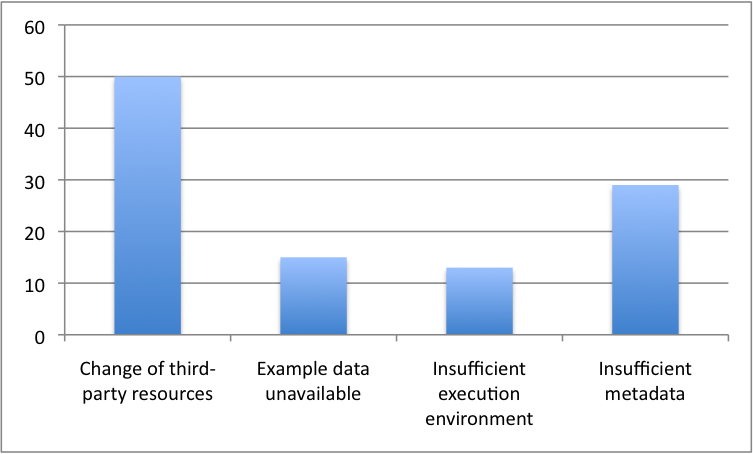
\includegraphics[width=9cm]{./Figures/decay_analysis_chart1-v2.png}
  \caption{A summary of workflow decay causes}
\end{subfigure}
\begin{subfigure}[t]{8cm}
  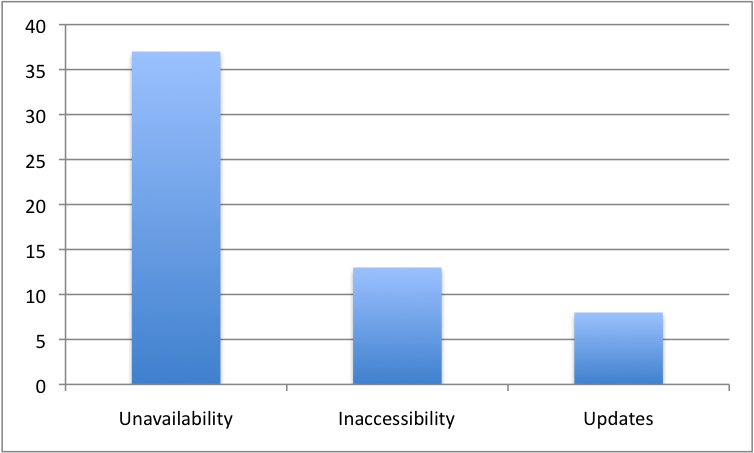
\includegraphics[width=7cm]{./Figures/decay_analysis_chart2-v2.png}
  \caption{Workflow decay due to third party resources}
\end{subfigure}
\caption{Results of workflow decay analysis.}
\label{fig:decay-analysis}
\end{figure}


% \begin{figure}[ht]
% \centering
% \subfigure[A summary of workflow decay causes.]{
% 	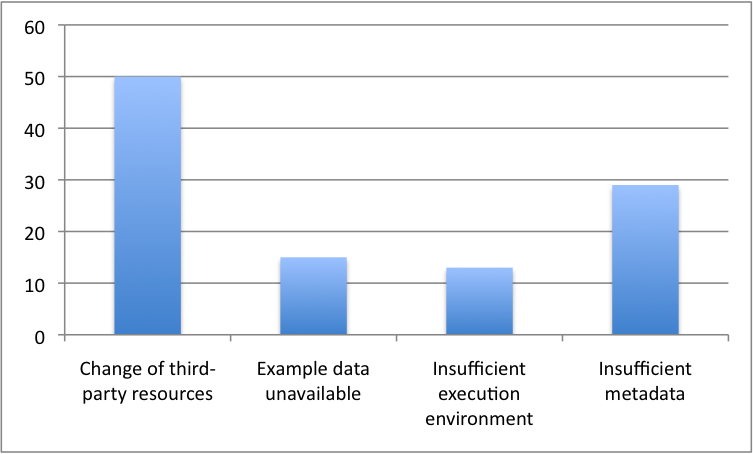
\includegraphics[width=9cm]{./Figures/decay_analysis_chart1-v2.png}
% }
% \subfigure[Workflow decay due to third party resources.]{
%     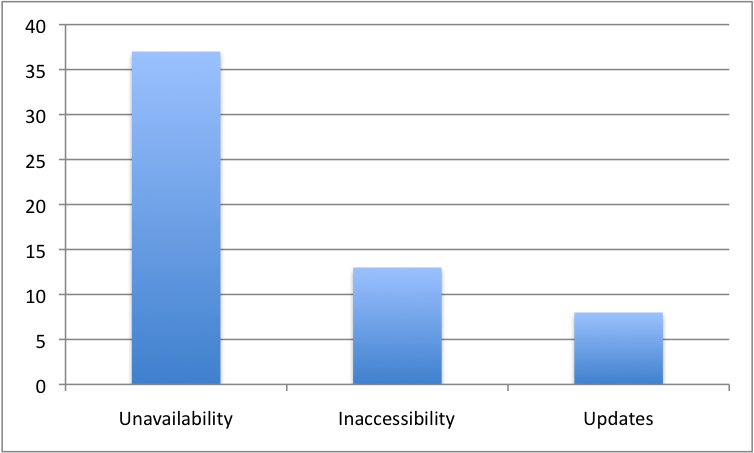
\includegraphics[width=7cm]{./Figures/decay_analysis_chart2-v2.png}
% }
% \caption{Results of workflow decay analysis.}
% \label{fig:decay-analysis}
% \end{figure}


To better understand the causes of decay due to third party resources. Figure \ref{fig:decay-analysis}-b illustrates the number of workflows that suffer from the causes presented in Table~\ref{table:decay}. It shows that the unavailability of third party resources is the leading cause of decay, followed by resources inaccessibility, and then resources changes. 

The above results confirms our hypothesis that workflow decay is a serious problem. It also suggests that there is a need for additional information that can assist workflow designers detecting and repairing decayed workflows. We report in a separate deliverable \cite{D4.2v1}, on a minimal model and associated checklists, that were designed and developed with the objective to prevent and repair workflow decay.


\appendix
\clearpage
\addcontentsline{toc}{section}{Bibliography}
\bibliographystyle{alpha}
\bibliography{refs.bib}
%------------------------------------------------------------------------------------------------------
%Keep following label in order for Latex to get the total number of pages right
%---
\label{lastpage}
%---
\end{document}
